\pdfoutput=1 % build with pdflatex
\documentclass[10pt,twocolumn]{article}
\PassOptionsToPackage{hyphens}{url} % break long URLs in narrow columns

\usepackage[T1]{fontenc}
\usepackage{lmodern} % scalable fonts so microtype expansion works
\usepackage[margin=1in]{geometry}
\usepackage{microtype}
\usepackage{booktabs}
\usepackage{graphicx}
\usepackage{tikz}
\usetikzlibrary{positioning, arrows.meta, fit}
\usepackage[numbers,sort&compress]{natbib}
\usepackage[colorlinks=true, allcolors=blue]{hyperref}
\usepackage{amsmath, amssymb, amsthm}
\theoremstyle{definition}
\newtheorem{definition}{Definition}
\newtheorem{assumption}{Assumption}
\setlength{\emergencystretch}{2em}

\title{From Privacy to Workflow Integrity:\\
Communication-Graph Metadata in Autonomous Agent Interoperability}
\author{Bijaya Dangol\\ Independent Researcher\\ \texttt{dangoldbj23@gmail.com}}
\date{\today}

\begin{document}
\twocolumn[%
  \begin{@twocolumnfalse}
  \maketitle
  \begin{abstract}
Agent-interoperability protocols such as A2A and MCP standardize what agents say to
one another, but assume address-based transport over HTTP(S). Such transports
protect message \emph{content}, increasingly with end-to-end encryption. What they
leave in the clear is the \emph{communication graph}: which agent contacts which,
when, and how often. In agent systems this graph is more consequential than a privacy
framing suggests. Endpoints are often capability-labeled, workflows are structured and
chained, and interactions are coupled to real actions, so an observer of the graph
recovers more than a history of past relationships. It can infer the \emph{pending
workflow}, the task being assembled and the action likely to follow, and, because
these workflows execute at machine speed, act on that inference before the workflow
completes. The threat is therefore one of \emph{workflow integrity}, not privacy
alone: predictive leverage over autonomous action.
We give a threat model for the agent communication graph; identify what makes agent
metadata distinctively revealing (semanticity, prospectivity, actuation); define
transport- and bootstrap-layer privacy properties (unlinkability, no central
observer, deniability, metadata minimization, and discovery privacy) and evaluate
candidate transports (SimpleX/SMP, Tor, mixnets) against them; and present an A2A
case study in which a metadata-protecting binding is expressible but surfaces the
protocol's implicit identity assumptions. We then test both claims on a generative
model of agent workflows anchored to a real A2A capture. From passive metadata alone,
with no payloads, a classifier recovers an interaction's task class well above chance,
and does so from only the opening of a workflow. Applied together, the properties
drive that recovery sharply back toward chance. Beyond what an observer can
\emph{recover}, we measure the leverage of acting on the leak: an adversary that must
choose, from a workflow's opening and under a fixed budget, which workflows to act on
realizes in this model most of the advantage a clairvoyant attacker would have over a
metadata-blind one, and the same properties that suppress inference suppress this
leverage.
  \end{abstract}
  \bigskip
  \end{@twocolumnfalse}
]

\section{Introduction}\label{sec:intro}
AI agents built by different vendors are increasingly made to interoperate through
open protocols. A2A~\citep{a2a}, now hosted by the Linux Foundation, and MCP~\citep{mcp} let agents
discover one another, delegate tasks, and increasingly transact on behalf of users and
organizations. These protocols standardize the \emph{content} and structure of agent
messages, but assume a conventional, address-based transport: agents are reachable
at URLs or stable names, and messages travel over HTTP(S).

Transport security here has focused, reasonably, on protecting message content: TLS
in transit and a growing set of end-to-end schemes that keep payloads from
intermediaries. What this leaves untouched is the \emph{communication graph}: the
record of which agent contacts which, when, how often, and how much data flows.
Because routing requires addressing and addresses are identifiers, this graph is
visible to network observers, relays, and registries even when every payload is
encrypted.

The graph is more than a privacy concern. Endpoints are often capability-labeled,
workflows are structured and chained, and interactions are coupled to real actions.
From such a graph an observer reads the \emph{shape of a task in progress}, not merely
a record of past contacts, and at machine speed can act on that shape before the
workflow completes. What is exposed is then a matter of \emph{integrity}, not privacy
alone: the observer holds predictive leverage over actions that have not yet occurred.
Existing agent-protocol threat models examine authentication, identity, and payload
leakage; the communication graph, with its prospective, action-coupled character, has
drawn little attention. This paper develops it systematically.

Our contributions are:
\begin{enumerate}
  \item A \textbf{threat model} for the agent-interop \emph{communication graph} as
  a metadata surface, separate from payload confidentiality
  (\S\ref{sec:threat}, \S\ref{sec:problem}).
  \item An account of \textbf{why agent metadata is distinctively revealing} (its
  semanticity, prospectivity, and actuation), which reframes the threat from privacy
  to the \emph{integrity of autonomous workflows} (\S\ref{sec:different}).
  \item A \textbf{transport- and bootstrap-privacy property framework} (unlinkability,
  no central observer, deniability, metadata minimization, and discovery privacy) and
  an evaluation of candidate transports against it (\S\ref{sec:properties},
  \S\ref{sec:transports}).
  \item An \textbf{A2A case study} showing a metadata-protecting binding is
  expressible but surfaces the protocol's implicit identity assumptions, and a
  \textbf{reconciliation} with the ecosystem's identity and reputation direction
  (\S\ref{sec:casestudy}, \S\ref{sec:discussion}).
  \item An \textbf{empirical evaluation} on simulated agent workflows anchored to a
  real A2A capture: a label-blind network observer recovers task class well above
  chance and from only a short prefix of a workflow, and only the full set of
  properties collapses this recovery toward chance; and, moving from inference to
  action, that the recovered signal carries decision-theoretic \textbf{leverage}: an
  adversary acting under a budget from a workflow's opening captures most of the
  attainable advantage over a blind baseline, which the same properties largely
  remove (\S\ref{sec:eval}).
\end{enumerate}

\section{Background}\label{sec:background}

\subsection{Agent interoperability protocols}
A2A models interoperation as \emph{tasks} exchanged between a client and a remote
agent. Agents publish \emph{Agent Cards} (metadata documents at well-known URLs
that declare capabilities, endpoints, and authentication) and communicate over one
of several \emph{bindings} (JSON-RPC, gRPC, or HTTP+JSON), all over
HTTPS~\citep{a2a}. Operations are asynchronous: a call returns immediately, and task
updates arrive by polling, server-sent streaming, or push notifications to a
client-provided webhook~\citep[\S3.1.7]{a2a}. A2A also admits \emph{custom protocol
bindings} for transports beyond the core set~\citep[\S5]{a2a}, the extension point
we use in \S\ref{sec:casestudy}. MCP plays a complementary
(agent-to-tool) role but shares the same address-based, HTTP-oriented assumptions.

\subsection{Transport security today}
Beyond TLS, recent bindings strengthen content protection: SLIM/SLIMRPC provides
broker-less delivery with MLS end-to-end encryption~\citep{slim, mls}, so that no
central intermediary reads message content. These mechanisms target confidentiality
and, for SLIM, the removal of a trusted broker; none aims at concealing the
communication graph.

\subsection{Metadata-protecting transports}
A separate lineage protects communication \emph{metadata}: mix
networks~\citep{chaum1981mix}, onion routing~\citep{tor}, mixnets~\citep{nym}, and
identity-less messaging such as SimpleX's SMP~\citep{simplex}. These were built for
human or general messaging; \S\ref{sec:transports} asks what they offer when
repurposed as agent-interop transports.

\section{System and Threat Model}\label{sec:threat}

\begin{figure*}[t]
\centering
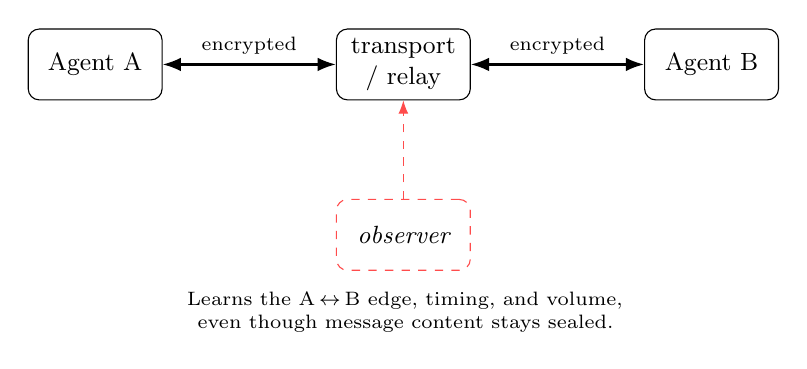
\begin{tikzpicture}[>=Latex, node distance=2.2cm,
  box/.style={draw, rounded corners, minimum width=1.7cm, minimum height=0.9cm,
              font=\small, align=center}]
  \node[box] (A) {Agent A};
  \node[box, right=of A] (R) {transport\\/ relay};
  \node[box, right=of R] (B) {Agent B};
  \draw[<->, thick] (A) -- node[above, font=\scriptsize] {encrypted} (R);
  \draw[<->, thick] (R) -- node[above, font=\scriptsize] {encrypted} (B);
  \node[box, draw=red!70, dashed, below=1.25cm of R, font=\small\itshape] (O) {observer};
  \draw[->, red!70, dashed] (O) -- (R);
  \node[below=0.15cm of O, font=\scriptsize, text width=6.4cm, align=center]
    {Learns the A\,$\leftrightarrow$\,B edge, timing, and volume, even though
     message content stays sealed.};
\end{tikzpicture}
\caption{Content encryption protects the payload but not the communication graph.
An observer at the network or at an intermediary learns who talks to whom, when, and
how often; in agent systems, often capability-labeled endpoints and their sequence
further reveal the task in progress (\S\ref{sec:different}).}
\label{fig:graph}
\end{figure*}

\subsection{System model}
We consider a set of agents $\mathcal{A}=\{a_1,a_2,\dots\}$ that interoperate by
exchanging messages under an interop protocol such as A2A or MCP. Two agents
communicate over a \emph{transport binding} that realizes the protocol's abstract
operations (request/response, streaming updates, and notifications) over a
concrete transport. A binding may route through one or more \emph{intermediaries}
(relays, gateways, or brokers), and the protocol may use a \emph{registry} for
capability discovery and connection bootstrap.

An \emph{interaction} between $a_i$ and $a_j$ is the set of messages exchanged to
complete one logical exchange (in A2A, the lifecycle of a task). Each message $m$
carries a transport-visible descriptor
\[
  \mathrm{obs}(m) = (\mathrm{src},\,\mathrm{dst},\,t,\,\ell,\,d),
\]
its endpoint identifiers, timestamp, length, and direction. Notably
$\mathrm{obs}(m)$ excludes the message \emph{content}, which we assume encrypted
(Assumption~\ref{asm:content}).

\subsection{The communication graph}
Over a period of operation, interactions induce a \emph{communication graph}
$G=(V,E)$: $V$ is the set of transport-visible agent identifiers, and each edge
$e\in E$ records that two endpoints interacted, annotated with timing, frequency,
and volume. A \emph{linkage} relation maps transport-visible identifiers to
persistent agent or operator identities. The assets we protect are $G$, this
linkage, and, as \S\ref{sec:different} argues, the predictive leverage over future
action that $G$ confers; not the content, which is protected by other means.

\subsection{Adversary model}
We model \emph{honest-but-curious} adversaries distinguished by vantage point
(Table~\ref{tab:adv}); the threat is that $G$ leaks without any active attack. A
network observer $\mathcal{N}$ sees $\mathrm{obs}(m)$ for messages on observed
links; an intermediary $\mathcal{R}$ sees what it forwards; a registry
$\mathcal{G}$ sees discovery lookups and connection bootstrap; a participating or
log-retaining endpoint $\mathcal{E}$ sees its own interactions, and more under
collusion. Adversaries may collude to widen their coverage of $E$. Our leakage analysis needs
only passive observation: the objective ranges from reconstructing $G$ to inferring
the pending workflow it encodes (\S\ref{sec:different}). \emph{Acting} on that
inference (to preempt or interfere) may require separate active capabilities,
which only strengthen the adversary.

\begin{table*}[t]
\centering\small
\begin{tabular}{@{}lll@{}}
\toprule
Adversary & Vantage point & Observes \\
\midrule
$\mathcal{N}$ network & links / paths & $\mathrm{obs}(m)$: endpoints, timing, volume \\
$\mathcal{R}$ intermediary & relay / gateway / broker & forwarded src/dst, timing, volume \\
$\mathcal{G}$ registry & discovery service & lookups, connection bootstrap \\
$\mathcal{E}$ endpoint / log & a participant or its logs & own interactions; more under collusion \\
\bottomrule
\end{tabular}
\caption{Adversary classes. All are passive (honest-but-curious) in the base
model and may collude to increase coverage of $E$.}
\label{tab:adv}
\end{table*}

\subsection{Trust assumptions and scope}
\begin{assumption}[Content confidentiality]\label{asm:content}
Message content is end-to-end encrypted under secure primitives; the adversary
learns nothing from payloads.
\end{assumption}
We deliberately grant the \emph{strongest} content protection so as to isolate the
metadata axis: any leakage we identify is leakage that content encryption, however
strong, does not prevent.
\begin{assumption}[No trusted graph custodian]\label{asm:nocustodian}
No single party is trusted to observe the full communication graph.
\end{assumption}
Out of scope are content confidentiality and payload data minimization (assumed
handled elsewhere), application-level authorization, and side channels outside the
transport.

\section{The Communication-Graph Metadata Problem}\label{sec:problem}

\subsection{Content and metadata are independent}
The starting point is a simple but consequential observation: content
confidentiality and communication-graph privacy are \emph{independent}, because
they protect different things. An interaction can be perfectly content-confidential
and still be fully graph-exposed.

Concretely, under Assumption~\ref{asm:content} the payload reveals nothing, yet
routing still requires the transport to address the destination. When endpoints
are named by persistent identifiers, those identifiers appear as $\mathrm{src}$
and $\mathrm{dst}$ in every $\mathrm{obs}(m)$ and directly reveal the edge; the
timing $t$, length $\ell$, and direction $d$ are visible regardless of encryption.
Since $G$ is by definition the set of such edges, any adversary that observes them
reconstructs $G$ no matter how strong the content protection is.

We state this as an observation, not a theorem, on purpose: it is close to
definitional. The contribution is not the claim that metadata leaks (that is well
understood for communication systems in general) but a systematic account of
\emph{which} metadata leaks in agent-interop protocols, to \emph{whom}
(\S\ref{sec:threat}), what a transport must provide to prevent it
(\S\ref{sec:properties}), and the protocol-level consequences of providing it
(\S\ref{sec:casestudy}).

\subsection{A walk through the A2A task lifecycle}
Let a client $a_c$ delegate a task to a server $a_s$ under A2A, with all content
encrypted. At \emph{discovery}, $\mathcal{G}$ observes that $a_c$ resolved $a_s$.
At \emph{connection setup}, $\mathcal{N}$ and any on-path $\mathcal{R}$ observe the
$a_c\!\leftrightarrow\!a_s$ edge. On \emph{message/send} they observe timing and
size; across \emph{streaming or polled updates} they observe cadence and volume; a
\emph{push notification} additionally exposes $a_c$'s callback endpoint. By
\emph{completion}, although no adversary has read a single field of the task,
$\mathcal{N}$, $\mathcal{R}$, and $\mathcal{G}$ jointly learn that $a_c$ engaged
$a_s$, when, how often, and how much data flowed, and across many tasks the
shape of the agents' relationships.

\subsection{Why current bindings do not address it}
The A2A bindings over HTTPS (JSON-RPC, gRPC, HTTP+JSON) protect content with TLS
but address agents by URL, so $\mathcal{N}$ and $\mathcal{R}$ obtain the edge
directly. SLIM/SLIMRPC removes the central content-reading broker via MLS, yet
routes by a persistent structured name; $\mathcal{R}$ and $\mathcal{N}$ still
obtain the edge, and the persistent name supplies the linkage of
\S\ref{sec:threat}. None of these target $G$: they protect content, which is
independent of the graph.

\subsection{Problem statement}
\begin{definition}[Metadata-protecting binding]\label{def:mpb}
A transport binding is \emph{metadata-protecting} against an adversary class if,
from that adversary's observations, it cannot reconstruct the communication graph
$G$, nor infer the pending workflow it encodes (\S\ref{sec:different}), beyond a
bounded, unlinkable view, as made precise by the properties of \S\ref{sec:properties}.
\end{definition}

\section{Why Agent Metadata Is Different}\label{sec:different}
Generic communication metadata reveals \emph{that} parties communicated. In agent
interoperability the same graph can reveal something stronger, a \emph{task in
progress}, because agent interactions differ from generic messaging along three
axes.

\paragraph{Semanticity.} Agent endpoints, tools, and registry entries are often
semantically meaningful rather than opaque addresses. Agent Cards advertise skills, registries are queried by capability, and
MCP tools are named by function. Observing that a client contacted a
``contract-review'' agent or invoked a ``payments'' tool reveals the \emph{class} of
task, not merely that an interaction occurred. This is the explicit-label analogue
of website-fingerprinting attacks, where the class of activity is inferred from
encrypted-traffic metadata~\citep{wfp}, except that here the label is advertised
rather than inferred. What an observer actually recovers depends on vantage point
and binding: a registry sees capability queries directly, whereas a pure network
observer may recover labels only indirectly, through discovery lookups, Agent Card
fetches, structured names, or repeated endpoint patterns.

\paragraph{Prospectivity.} Agent workflows are structured and chained: discovery
precedes delegation, delegation precedes tool invocation, and updates follow. Early
steps can therefore predict later ones. An observer who recognizes the opening of a
familiar workflow may anticipate its trajectory before it completes, rather than
learning of it only afterward.

\paragraph{Actuation.} Agent interactions often \emph{trigger actions} directly,
without a human reviewing each step. The graph is thus coupled to consequences in
the world: influencing or interrupting the observed workflow can change what the
agents actually do.

As an illustration, a lookup for a sanctions-screening agent, followed by
payment-settlement and contract-review calls, suggests a cross-border transaction
being assembled, revealing the \emph{kind} of deal in progress well before it
completes, without a single payload being read.

Together these shift the adversary's objective. From passive observation alone a
graph observer may infer historical relationships and, beyond them, \emph{pending
intent and workflow trajectory}. The \emph{harm} comes when the adversary acts on
that inference through separate, active channels: poisoning discovery, preempting a
negotiation, triggering a competing action. Because the workflow is structured and
runs at machine speed, such a move can land before the workflow completes. The
pattern is familiar from front-running in decentralized exchanges, where adversaries
watch pending-transaction metadata and act ahead of it~\citep{flashboys}. Agent
interoperability raises the analogous risk wherever workflows are capability-labeled
and structured, and potentially across many application domains rather than one.

The framing shifts accordingly. Protecting the communication graph is not merely a
privacy question, concealing who interacts; it concerns the \emph{integrity and contestability
of autonomous workflows}: their freedom to execute, and to be steered by their
principals rather than by an outside observer who holds predictive leverage over
machine-speed action. Section~\ref{sec:eval} measures how much intent the graph
leaks, inferring task class from endpoint and sequence metadata; here the threat
serves as the design motivation. A scope note: what becomes transport-visible is
\emph{inter-agent and inter-tool} coordination, not an agent's internal, local
planning.

\section{Privacy Properties for Transport and Bootstrap}\label{sec:properties}
The following properties span transport and bootstrap and are protocol-independent;
for each we note the adversary capability it removes.

\begin{definition}[Unlinkability]\label{def:unlink}
An adversary cannot tell whether two observed interactions involve the same agent,
nor link a transport-visible identifier to a persistent agent identity. This
requires that identifiers not be stable across interactions: each interaction uses
a fresh identifier unlinkable to the agent's others.
\end{definition}
\noindent Identifier freshness is the mechanism; it denies the edge-linkage of
\S\ref{sec:threat} to $\mathcal{N}$ and $\mathcal{R}$, and the persistent-identity
linkage to all classes.

\begin{definition}[No central observer]\label{def:nocentral}
No single adversary vantage point observes more than a small fraction of $E$;
reconstructing $G$ requires collusion among multiple independent parties.
\end{definition}
\noindent This targets the global view of a network observer $\mathcal{N}$ or a
shared intermediary $\mathcal{R}$, and follows Assumption~\ref{asm:nocustodian}.

\begin{definition}[Deniability]\label{def:deny}
An interaction leaves no transferable transcript that cryptographically binds a
specific agent to participation; any party can plausibly deny it.
\end{definition}
\noindent This targets a logging or colluding endpoint $\mathcal{E}$.

\begin{definition}[Metadata minimization]\label{def:minimize}
The observable descriptors $(t,\ell,d)$ are reduced (e.g., padded, batched, or
mixed) so that timing and volume do not distinguish interactions.
\end{definition}
\noindent This targets traffic analysis by $\mathcal{N}$ and $\mathcal{R}$ that
survives even fresh identifiers.

\begin{definition}[Discovery privacy]\label{def:discovery}
Capability lookup and connection bootstrap do not reveal the requested capability,
the selected peer, or the resulting interaction edge to an untrusted registry or
transport intermediary.
\end{definition}
\noindent This targets the registry $\mathcal{G}$ and the early, pre-interaction
leakage that \S\ref{sec:different} identifies as especially sensitive.

Definitions~\ref{def:unlink}--\ref{def:minimize} are wire-transport properties;
\S\ref{sec:transports} evaluates how far real transports meet them. Discovery
privacy (Definition~\ref{def:discovery}) is realized at the bootstrap layer instead,
and \S\ref{sec:casestudy} shows how an identity-less binding can provide it through
out-of-band exchange. Together they make a binding metadata-protecting
(Definition~\ref{def:mpb}) against the corresponding adversaries; in the terms of
\S\ref{sec:different} they bound an adversary's predictive leverage by denying the
identity, timing, and discovery cues that make workflow inference possible, so they
protect the integrity of autonomous workflows, not only privacy.

\section{Transport Design Space}\label{sec:transports}
No transport was designed for agent interoperability; each was built for human or
general messaging, so applying it inherits both its protections and its
limitations. Table~\ref{tab:transports} rates candidate transports against the
properties of \S\ref{sec:properties}, alongside the HTTP(S) and SLIM bindings as
baselines. Ratings are qualitative (\emph{strong} / \emph{partial} /
\emph{weak}); the point is the shape of the trade-off, not a score.

\begin{table*}[t]
\centering\footnotesize
\begin{tabular}{@{}lccccl@{}}
\toprule
Transport & Unlinkability & No central obs. & Deniability & Metadata min. & Cost \\
\midrule
HTTP(S) / current bindings & weak & weak & weak & weak & low latency, mature \\
SLIM / SLIMRPC & weak & partial & weak & weak & low latency, maturing \\
SimpleX / SMP & strong & strong & strong & partial & async, modest throughput \\
Tor onion services & weak & strong & partial & partial & moderate latency, mature \\
Mixnet (e.g.\ Nym) & strong & strong & strong & strong & high latency, emerging \\
\bottomrule
\end{tabular}
\caption{Candidate transports rated against the four wire-transport properties of
\S\ref{sec:properties}; discovery privacy is a bootstrap-layer concern, addressed in
\S\ref{sec:casestudy}. Ratings are qualitative; the point is the trade-off, not a
score.}
\label{tab:transports}
\end{table*}

\paragraph{HTTP(S) bindings (incl.\ SLIM).} Agents are addressed by persistent URL
or structured name, so unlinkability is weak and a network observer or intermediary
obtains the edge directly. SLIM removes the central content-reading broker (an
improvement over a single shared intermediary) but still routes by persistent
name and provides no identifier freshness, mixing, or deniability.

\paragraph{SimpleX / SMP.} Identity-less by construction: connections are
bootstrapped out of band and carried over unidirectional queues with per-queue
identifiers and no global account, giving strong unlinkability and, with separate
and rotating relays, no single observer of the graph; deniability is a design goal.
Its weak point is metadata minimization (a relay still sees the timing and volume
of the queues it hosts), so traffic-analysis defenses are only partial. The model
is asynchronous with modest throughput.

\paragraph{Tor onion services.} Strong at hiding network location and distributing
trust across relays, but a published onion address is a \emph{persistent}
identifier, so unlinkability is weak when agents reuse addresses, and a global
passive adversary can mount traffic correlation. Maturity is high, latency
moderate.

\paragraph{Mixnets (e.g.\ Nym).} Purpose-built for metadata protection: per-packet
unlinkable formats, distributed mixing, and cover traffic earn strong ratings on
unlinkability, no-central-observer, and metadata minimization. The cost is high
latency and lower maturity, precisely the trade-off a deployment must weigh.

\paragraph{Takeaway.} No transport provides all four wire-transport properties
cheaply; they trace a privacy/latency frontier. SMP is a strong first instantiation because it is
identity-less and ships today; a mixnet is stronger on traffic analysis at a
latency cost; Tor is the most mature but weakest on unlinkability. The properties
of \S\ref{sec:properties}, not any single transport, are the portable target.

\section{Case Study: A Metadata-Protecting Binding for A2A}\label{sec:casestudy}
A2A is a useful case study because it already admits transports beyond its core set
through \emph{custom protocol bindings}, and because its operations are already
asynchronous: an operation returns immediately and updates arrive by polling,
streaming, or push. A metadata-protecting binding is therefore expressible in
principle. The instructive result is what one meets in trying: mapping A2A onto an
identity-less transport (we use SMP) surfaces three \emph{implicit identity
assumptions} that the specification never states because, over HTTP, they always
hold.

\paragraph{Assumption 1: push notifications assume an HTTP-reachable client.}
A2A push delivers task updates to a client-provided webhook URL~\citep[\S3.1.7]{a2a},
presuming the client has a stable, reachable address; an identity-less client has
none. This is
\emph{surmountable}: server-initiated delivery re-maps onto the transport's own
asynchronous channel. At task creation the client supplies a reply queue it
controls, and the server posts updates there. Because A2A already treats push as one
of several interchangeable update mechanisms, the semantics are preserved; only the
carrier changes.

\paragraph{Assumption 2: authentication is identity-based.}
A2A authentication is declared in the Agent Card and is identity-bearing (mutual
TLS~\citep[\S4.5.6]{a2a}, OAuth/OIDC, keys tied to a principal). An identity-less transport cannot
present a stable principal. This is the \emph{genuine mismatch}: schemes that
require a verifiable persistent identity (a client certificate, an OIDC subject) do
not translate. What does translate is a different trust basis: channel binding from
the out-of-band handshake, plus capability- or credential-based authorization via
selectively disclosed attestations (\S\ref{sec:discussion}). This establishes
\emph{what} a peer is entitled to without fixing \emph{who} it persistently is.

\paragraph{Assumption 3: discovery assumes addressable endpoints.}
A2A discovery resolves an Agent Card at a well-known URL~\citep{a2a} and selects a
binding from its declared endpoint. With no addressable endpoint, both the card's location and
the endpoint it advertises must change form. This is \emph{surmountable} but needs a
different bootstrap: capabilities are exchanged out of band (an invitation carries or
precedes the Agent Card), and the card declares a rendezvous or invitation mechanism
in place of a URL. The capability \emph{content} of the card is unaffected; its
addressing model is what gives way.

\paragraph{What the case study shows.} Two of the three assumptions (push,
discovery) are surmountable by re-mapping onto asynchronous and out-of-band
mechanisms the transport already provides; one (identity-based authentication) is a
semantic mismatch that forces a different, credential-based trust basis. None is
stated in the specification, because over an address-based transport they hold for
free. Naming them is useful independently of whether an identity-less binding is
ever standardized: they delimit exactly where interoperability and persistent
identity are entangled. They are also where an adversary would act: discovery and
push are the early, action-coupled steps whose visibility enables the preemption of
\S\ref{sec:different}.

\section{Empirical Evaluation}\label{sec:eval}
Two claims from the earlier sections invite a test. The threat model holds that graph
metadata leaks \emph{pending workflow intent} (\S\ref{sec:different}); the property
framework holds that a defined \emph{set} of properties removes it
(\S\ref{sec:properties}). We evaluate both, and then ask the third, decision-theoretic
question the integrity framing demands: what the recovered signal is \emph{worth} to
an adversary that acts on it (\S\ref{subsec:actuation}). The aim is a controlled demonstration
rather than a field measurement: that intent is recoverable from passive metadata,
that it is recoverable \emph{early}, and that the properties reduce recovery sharply
toward chance, and only in combination.\footnote{Code and data:
\url{https://github.com/dangoldbj/agent-metadata-privacy}.}

\subsection{Setup}
No public corpus of agent-interop traces exists, so we sample workflows from a
generative model of the A2A task lifecycle: discovery, delegation, streamed updates,
completion. Each \emph{task class} is a stochastic process over capability-typed
stages, drawn from a shared vocabulary with tunable overlap, so the \emph{set} of
capabilities alone does not identify the class. Several agents serve each capability
and some are multi-skill, so a transport-visible identifier is \emph{not} merely a
relabeled capability. Timing and size profiles attach to capabilities rather than
classes and are shared across them; all class signal therefore flows through
\emph{which} capabilities are invoked and \emph{in what order}. Each message yields
the descriptor $\mathrm{obs}(m)$ of \S\ref{sec:threat}, and content is never observed.
To check realism, we anchor the generator to a real capture from the A2A reference
SDK, a live task lifecycle driven over HTTP, and confirm that it matches the
lifecycle's structure and scale.

An \emph{adversary view} projects a trace onto what a single vantage point sees
(Table~\ref{tab:adv}). The \emph{registry} view sees the semantic capability labels
named in discovery queries. The \emph{network} view sees only opaque endpoint
identifiers, timing, volume, and direction, and no semantic labels. A classifier then
predicts the latent task class. Following the website-fingerprinting
tradition~\citep{wfp}, we treat its accuracy above chance as a conservative indicator
of leakage: an unoptimized decoder can only understate it, so we deliberately leave it
untuned. Chance is $1/K$ for $K$ balanced classes, and we
report cross-validated accuracy with a bootstrap $95\%$ confidence interval.

\subsection{Leakage is recoverable in the model, and prospective}
With $K=8$ balanced classes, chance is $0.125$. The registry view recovers the task
class at $1.00$, near-tautologically, since it observes the labels directly. The
result that matters is the \emph{label-blind} network view, which recovers the class
at $0.99$ (Fig.~\ref{fig:leakage}). An observer of pure transport metadata is thus
nearly as informed as one reading the advertised labels: persistent identifiers,
together with capability-correlated timing and volume, let it reconstruct the
capability footprint indirectly. This is the semanticity of \S\ref{sec:different} made
concrete.

Recovery is also \emph{prospective}. Given only the first tenth of a workflow, the
network view already predicts its class at $0.70$, roughly $5.6\times$ chance, and
accuracy climbs toward certainty as more of the workflow is observed
(Fig.~\ref{fig:prospectivity}). The opening of a workflow predicts its trajectory,
exactly the predictive leverage \S\ref{sec:different} singles out as distinctive to
agent metadata.

\begin{figure}[t]
\centering
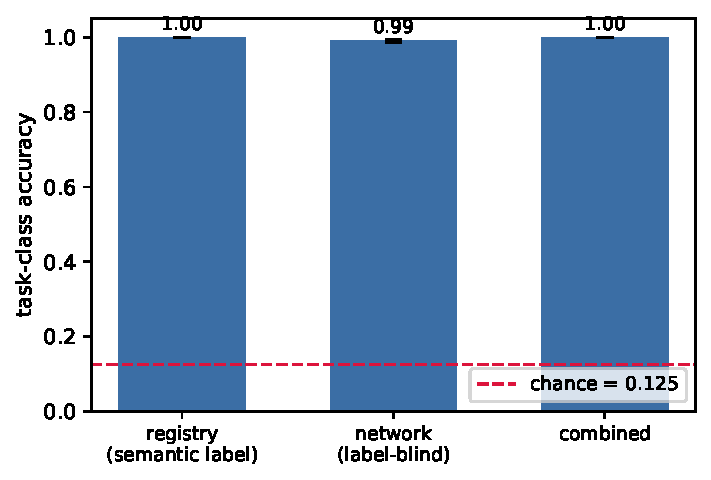
\includegraphics[width=\columnwidth]{figures/fig_leakage.pdf}
\caption{Task class recovered from communication-graph metadata, by adversary view
($K=8$, chance $0.125$; error bars are bootstrap $95\%$ CIs). Even the label-blind
\emph{network} view, seeing only $\mathrm{obs}(m)$, recovers the class far above
chance.}
\label{fig:leakage}
\end{figure}

\begin{figure}[t]
\centering
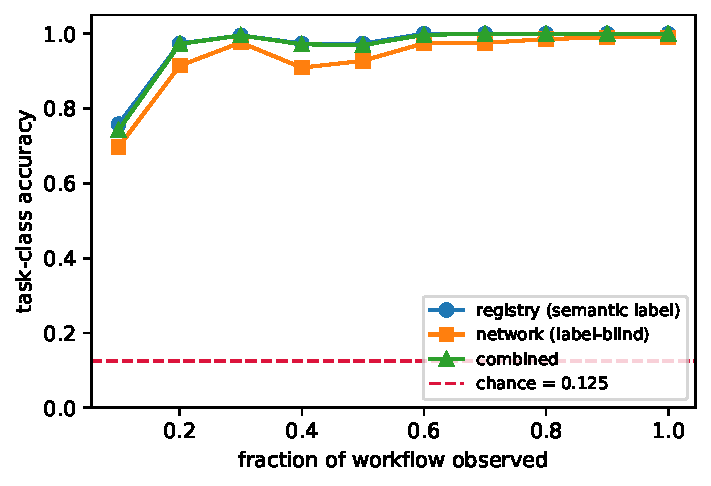
\includegraphics[width=\columnwidth]{figures/fig_prospectivity.pdf}
\caption{Prospectivity: accuracy as a function of the fraction of the workflow
observed. From only its opening, the network view predicts the pending task class
well above chance.}
\label{fig:prospectivity}
\end{figure}

\subsection{The properties neutralize the leak, but only as a set}
We next realize the properties of \S\ref{sec:properties} as transforms on the
observed traffic and re-measure (Fig.~\ref{fig:protection}). On its own, each wire
property barely moves the network observer. \emph{Unlinkability} (fresh
per-interaction identifiers) closes the persistent-identifier channel but leaves the
timing and volume fingerprint, holding accuracy at $0.95$. \emph{Metadata
minimization} (padding and a batched cadence) closes timing and volume but leaves the
identifiers, holding it at $0.99$. Only the two together collapse recovery, to
$0.42$. The registry view is a separate channel: neither wire property touches it,
and it falls only to \emph{discovery privacy} ($1.00\to0.125$, exactly chance). The
threat therefore yields only to the full \emph{set} of properties, each matched to a
channel; partial measures do not suffice, a content-protecting binding that retains
persistent names being one such case (\S\ref{sec:problem}). The residual $0.42$ stays
above chance because a
\emph{structural} channel remains: the message counts and sequence shape that the
wire properties do not target and that cover traffic would address
(\S\ref{sec:transports}).

\begin{figure}[t]
\centering
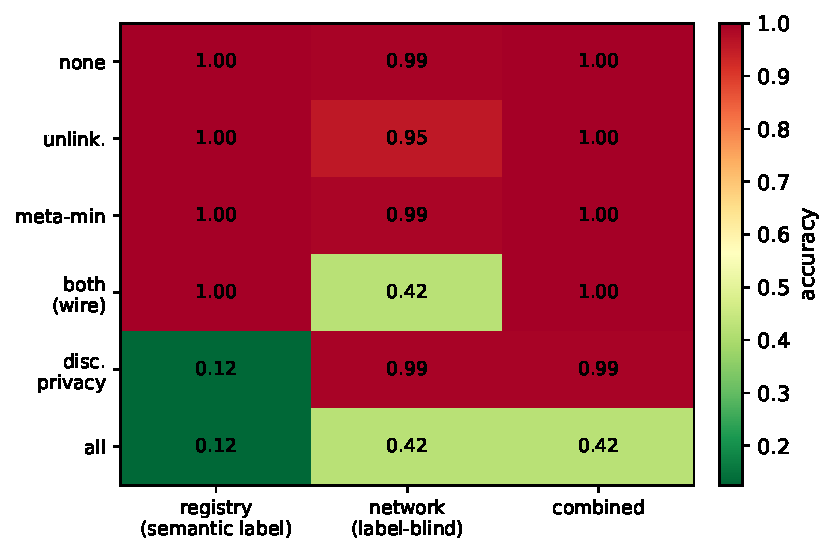
\includegraphics[width=\columnwidth]{figures/fig_protection.pdf}
\caption{Accuracy under each property (rows) for each adversary view (columns); red
is leaking, green is protected. The network observer falls only when unlinkability
and metadata minimization are combined (``both''); the registry observer falls only
to discovery privacy. No single property suffices.}
\label{fig:protection}
\end{figure}

\subsection{Actuation: the value of acting on the leak}\label{subsec:actuation}
Leakage and prospectivity are properties of recoverability: how much the metadata
tells an observer about the task. Whether that knowledge bears on workflow
\emph{integrity} is a separate, decision-theoretic question, since an observer that
cannot act on what it learns poses no integrity threat. We therefore model an
adversary that must \emph{act} under a budget and measure what the metadata is worth
to it.

\begin{definition}[Actuation game and value of metadata]\label{def:vom}
Among $N$ concurrent workflows, each $w$ carries an adversary value $v(w)\ge 0$. By a
decision deadline $f$, having observed only the leading fraction $f$ of every
workflow, a metadata-only adversary commits a budget of $B$ interventions, choosing a
set $S$ with $|S|=B$ to maximize $J(S)=\sum_{w\in S} v(w)$, and ranks workflows using
the label-blind network view of the observed prefix alone. With $J_{\mathrm{inf}}$,
$J_{\mathrm{blind}}$, and $J_{\mathrm{orc}}$ the objective under the
metadata-informed, uniformly random, and true-value selections, the \emph{value of
metadata} is $\mathrm{VoM}(B,f)=J_{\mathrm{inf}}-J_{\mathrm{blind}}$ and the
\emph{capture ratio} is
$\kappa=(J_{\mathrm{inf}}-J_{\mathrm{blind}})/(J_{\mathrm{orc}}-J_{\mathrm{blind}})$,
normalized so that $0$ is the blind baseline and $1$ the oracle; a ranking worse than
random can fall below $0$, and in our experiments $\kappa\in[0,1]$. It is the share of
the attainable advantage the adversary realizes from metadata alone.
\end{definition}

We instantiate the game minimally, adding nothing to the generator. One task class is
the adversary's target, $v(w)=1$ if $w$ is of that class and $0$ otherwise; the budget
equals one class's mass; the ranking is the network observer's out-of-fold posterior
on the target, from exactly the prefix features used in the preceding subsections. Then
$J_{\mathrm{inf}}$ is the count of true target workflows among the top-$B$ by that
posterior, and $J_{\mathrm{blind}}$ and $J_{\mathrm{orc}}$ are closed-form; we average
over the choice of target. What $\mathrm{VoM}$ and $\kappa$ capture is \emph{selection}
leverage: the advantage of picking the right workflows to act on, from the opening
alone. That is the precondition for changing outcomes, not proof that they change;
the latter would mean acting against a live binding (\S\ref{sec:discussion}).

The value of metadata is substantial and, like the inference beneath it, prospective.
Deciding from only the opening fifth of each workflow, the adversary captures
$\kappa\approx0.90$ of the attainable advantage over the blind baseline
(Fig.~\ref{fig:actuation}); from only the first tenth it already captures about
two-thirds, climbing toward unity as more of the workflow is seen
(Fig.~\ref{fig:actsep}, left). Under a budget, knowing the task early is most of the
way to acting on it.

Actuation is not a restatement of leakage. The value of metadata is the product of two
independent factors (an early-decidable signal and a budget to spend), and
collapses if either is absent: with no budget there is nothing to actuate, so
$\mathrm{VoM}\to0$ as the budget shrinks (Fig.~\ref{fig:actsep}, right), and with no
early signal the ranking is uninformative and $\kappa\to0$. The axis is genuinely
separate from recoverability, and website-fingerprinting, which bounds the signal
factor alone, does not speak to it.

The defense carries over, and again only as a set. Each wire property alone leaves the
leverage near its unprotected level ($\kappa=0.83$ under unlinkability, $0.92$ under
metadata minimization); the two together drive it to $0.12$, essentially the blind
baseline (Fig.~\ref{fig:actuation}). Notably the leverage falls further than inference
itself: under both properties the label-blind observer still recovers task class at
$0.42$ (Fig.~\ref{fig:protection}), yet that residual labeling power buys almost no
leverage, because selecting the highest-value workflows under a tight budget demands a
precision the residual channel lacks. Discovery privacy, which does not touch the
network view, leaves $\kappa$ unchanged, as expected. Selection leverage is downstream
of inference: with recovery gone, there is nothing left to target. The integrity defense
thus follows from the privacy defense, since the properties that suppress what an
observer can recover suppress the leverage it gains.

\begin{figure}[t]
\centering
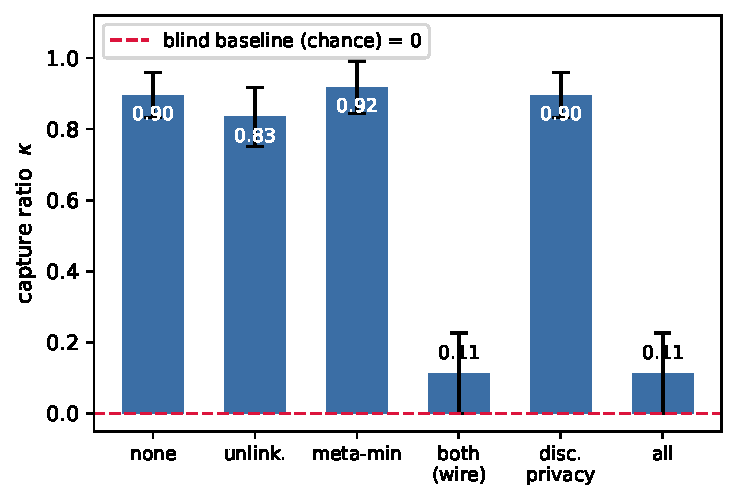
\includegraphics[width=\columnwidth]{figures/fig_actuation.pdf}
\caption{Actuation. Capture ratio $\kappa$ by privacy property, at an early decision
deadline ($f=0.2$) and a budget equal to one task class's mass, averaged over targets
(error bars span $\pm1.96$ standard errors across target classes; chance, the blind
baseline, is $0$). The
integrity analogue of Fig.~\ref{fig:protection}: only the combined wire properties
(``both'') collapse the leverage, and discovery privacy, which the label-blind
observer ignores, does not.}
\label{fig:actuation}
\end{figure}

\begin{figure*}[t]
\centering
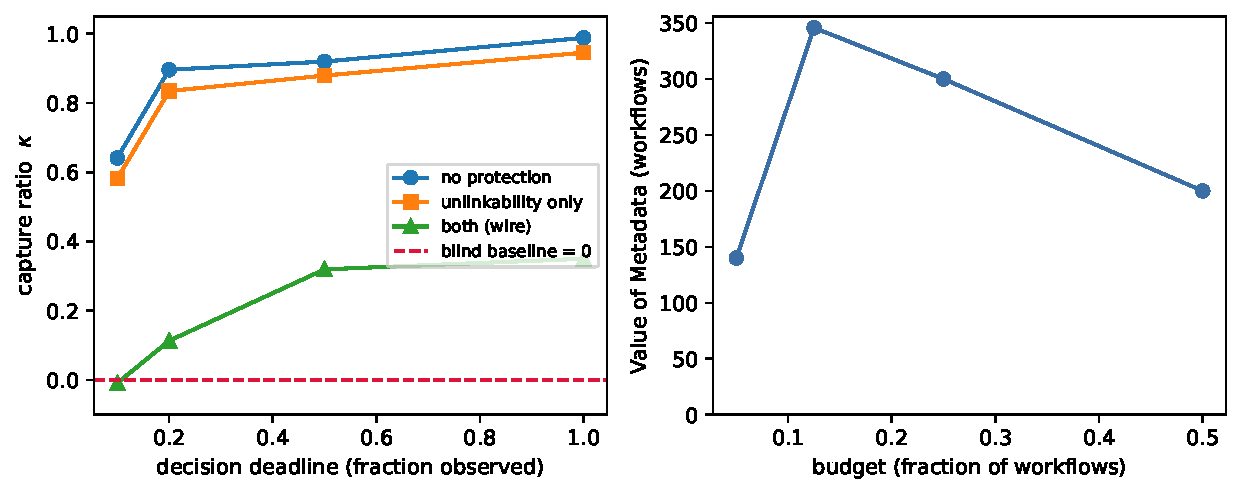
\includegraphics[width=\textwidth]{figures/fig_actuation_separation.pdf}
\caption{Actuation is the product of inference and budget, vanishing on either edge.
Left: capture ratio against the decision deadline; leverage tracks prospectivity, is
substantial even from a short prefix, and the combined wire properties hold it at the
blind baseline. Right: value of metadata against budget (no protection, full
workflow); it vanishes without a budget to spend and peaks where the budget is scarce
relative to the target set, the signature of a value-of-information quantity.}
\label{fig:actsep}
\end{figure*}

\subsection{Robustness and scope}
The effect is structural rather than tuned. Across sweeps of the number of classes,
the capability overlap, and the timing noise, the network view stays $4$--$14\times$
above chance, the short-prefix prediction stays above chance, and the two wire
properties always collapse recovery. We therefore claim the \emph{structure} of the
effect, not its precise magnitude; this holds for the value of metadata too. Two limitations
are intrinsic. The workflows are simulated and calibrated to a small real capture
rather than a labeled real corpus, so the magnitude is generator-dependent. And the
actuation result (\S\ref{subsec:actuation}) measures leverage \emph{in the model}: it
quantifies the advantage a budgeted adversary's selection gains from metadata over the
simulated workflow population, the decision-theoretic core of the integrity threat,
but stops short of a live exploit against a deployed binding. The evaluation thus
substantiates all three axes (semanticity, prospectivity, and actuation) and the
efficacy of the properties against each; demonstrating end-to-end manipulation on real
agent traffic is the natural next step.

\section{Discussion}\label{sec:discussion}

\subsection{Reputation and trust without a global graph}
A natural objection, especially in the current agent ecosystem, is that trust and
reputation require persistent identity and an observable history of interactions,
which metadata privacy appears to break. The tension is real but narrower than it
first appears. It conflicts only with \emph{global-observation} reputation: a
registry or ledger that watches all interactions to compute scores. That design is
fundamentally incompatible with unlinkability, and is itself a graph-surveillance
mechanism, i.e.\ the very asset of \S\ref{sec:threat}. It is compatible, however,
with two other models. Under \emph{credential-based} reputation, portable signed
attestations are selectively disclosed: an agent proves ``a verifier attests that I
completed $N$ tasks at quality $q$'' without revealing whom it transacted with, so
trust travels with the agent rather than being reconstructed from observed traffic.
Under \emph{pairwise} reputation, two agents accrue trust over their own repeated
interactions with no global observer. Both align with the verifiable-credentials
direction already pursued in the ecosystem; only the global-ledger variant
conflicts, and credential-based approaches can provide privacy-preserving
alternatives while preserving the properties of \S\ref{sec:properties}. This is also the trust basis that the authentication
mismatch of \S\ref{sec:casestudy} requires.

\subsection{Limitations}
The properties of \S\ref{sec:properties} are stated qualitatively; tightening them
into adversary-indistinguishability games is future work. The strongest metadata
protection (mixing, cover traffic) carries latency and bandwidth costs that may be
unacceptable for interactive, low-latency agent calls; an identity-less transport
also makes discovery and authentication harder, as \S\ref{sec:casestudy} shows.
Our evaluation (\S\ref{sec:eval}) measures inference and in-model actuation on
simulated workflows anchored to a real capture; a reference binding with live wire
measurements (latency, throughput, and an adversary's reconstruction of $G$ on real
traffic), and a demonstration of actuation against live agent traffic rather than
within the model, are the natural next steps.

\subsection{Deployment}
Because A2A exposes custom protocol bindings, a metadata-protecting binding can be
introduced incrementally and selected per Agent Card, coexisting with HTTP and SLIM
bindings rather than replacing them. Agents for which the communication graph is
sensitive (regulated, competitive, or adversarial settings) can opt in, while
latency-sensitive agents retain existing bindings. The threat model and properties
are transport- and protocol-agnostic, so the same analysis applies to MCP and to
other transports on the frontier of \S\ref{sec:transports}.

\section{Related Work}\label{sec:related}

\paragraph{Threat modeling of agent-interop protocols.}
Recent work has begun to systematize agent-interop security. Comparative threat
models examine MCP, A2A, Agora, and ANP for protocol-specific and cross-protocol
risks~\citep{threatmodel2026, secanalysis2025}, and surveys map the
interoperability landscape~\citep{survey2025}. These analyses concentrate on
authentication, identity, message injection, permissioning, and the leakage of
sensitive \emph{payload} data: for instance, the sensitive context streamed during
delegation~\citep{a2adata}. Our surface is
complementary
and, to our knowledge, not previously treated as a first-class transport-layer
security surface: the transport-level \emph{communication graph} (who communicates
with whom, when), which persists even when payloads are fully protected.

\paragraph{Privacy leakage in multi-agent systems.}
A parallel line studies information leakage \emph{within} multi-agent systems,
showing that inter-agent channels leak substantially more than output channels and
that privacy controls must extend to inter-agent
communication~\citep{agentleak2026, mas2025}. That work targets content-level
leakage between agents; we target the metadata of the interactions themselves at
the transport.

\paragraph{Anonymous communication.}
The properties we require (unlinkability, no central observer, metadata
minimization) originate in the anonymous-communication literature: mix
networks~\citep{chaum1981mix}, onion routing~\citep{tor}, and modern mixnets such as
Nym~\citep{nym}, surveyed broadly in~\citep{anoncomm}. Our contribution is not a new
anonymity system but the application of these properties to agent-interop transport
and an analysis of what an interop protocol must give up to obtain them
(\S\ref{sec:casestudy}).

\paragraph{Inference and preemption from metadata.}
That metadata enables \emph{semantic} inference is established for encrypted traffic
by website-fingerprinting attacks~\citep{wfp}; that observable pending intent enables
\emph{preemption} is established by front-running and miner-extractable value in
decentralized exchanges~\citep{flashboys}. We argue (\S\ref{sec:different}) that
agent interoperability combines both, at machine speed, and our actuation result
(\S\ref{subsec:actuation}) makes the bridge between them measurable: it casts the
\emph{value} of acting on recovered metadata as a decision-theoretic quantity (the
advantage a budgeted adversary gains over a blind baseline), distinct from
recoverability, and shows that a transport defense must drive that value down, not
merely reduce recovery. We draw on these literatures for the inference and preemption
primitives rather than extend them.

\paragraph{Credentials and unlinkability.}
The reconciliation of \S\ref{sec:discussion} draws on selectively disclosed
verifiable credentials, whose unlinkable presentation is an active area; the W3C
threat model for decentralized credentials catalogs the relevant attack
surfaces~\citep{w3ccred}. These mechanisms supply trust without a global interaction
graph, complementing the transport-level properties developed here.

\section{Conclusion}\label{sec:conclusion}
The communication graph of interoperating agents remains exposed under today's
address-based bindings even with end-to-end payload encryption, and in agent
systems it is more revealing than a privacy framing suggests. Because endpoints are often
capability-labeled, workflows are structured, and interactions are action-coupled,
the graph can leak \emph{pending} workflows and hand an observer predictive leverage
over machine-speed action. The exposure runs to the integrity and contestability of
autonomous workflows, not their privacy alone. We gave a threat model for this
surface, an account of what makes agent metadata distinctively revealing, transport-
and bootstrap-layer properties against which any binding can be evaluated, an A2A
case study in which pursuing those properties both surfaces and is constrained by the
protocol's implicit identity assumptions, and an empirical evaluation showing that
the leakage is real and prospective, that this leakage carries decision-theoretic
leverage (value to a budgeted adversary acting from a workflow's opening), and
that the properties, applied together, suppress both. A reference binding with live
measurements, and a demonstration of actuation against live agent traffic rather than
within the model, remain open.

\bibliographystyle{plainnat}
\bibliography{references}

\end{document}
